%!TEX root = ../Master.tex

\section{Test} % (fold)
\label{sec:test}

This section presents the results of testing the success rate of the Particle Filter implementation for localization. Since the code was not successfully executed on the physical robot platform, the tests have only been carried out as simulations using the visualization tool included in ROS.\\

The map used for the tests is shown in \autoref{fig:pf_test_init} where the initial location of the robot is on the right side of the map and the goal location is on the left side just below the small black box.

\begin{figure}[H]
\centering
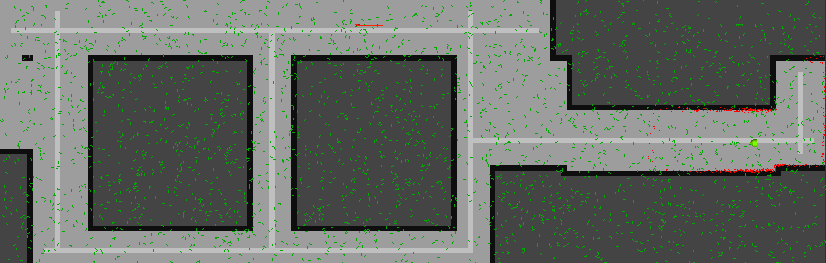
\includegraphics[scale=0.45]{images/pf_test_init}
\caption{Particle Filter Test - Robots start location}
\label{fig:pf_test_init}
\end{figure}

As mentioned, the objective of the test is to assess the success rate of the Particle Filter implementation for locating the robot. It is not always the case, that the Particle Filter leads the robot to finding the correct location, but instead, particle clusters gets formed at locations which are symmetric to the robots actual location. If this happens, the robot can actually start path planning from a wrong location, which either successfully reaches the goal in rare situations or if the particle cluster becomes sufficiently inconsistent with the actual robots distance measurements, the robot can get stuck because it is navigating the planned path with a wrong belief about its location and is therefore getting confused by the measurements it acquires.\\

\autoref{fig:pf_test_not_found_following_path} show the unfortunate situation where the wrong location becomes the posterior belief about the robots location and because the variance between the particles in the cluster is sufficiently small, a path is planned from this location to the goal.

\begin{figure}[H]
\centering
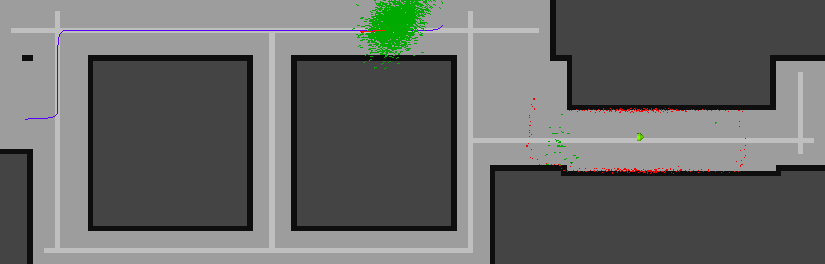
\includegraphics[scale=0.45]{images/pf_test_not_found_following_path}
\caption{Particle Filter Test - Wrong posterior belief}
\label{fig:pf_test_not_found_following_path}
\end{figure}

\autoref{fig:pf_test_robot_stuck} is an example of how the situation described above can result in the robot getting stuck because it is trying to follow the blue path, but with a false belief about the robots location.

\begin{figure}[H]
\centering
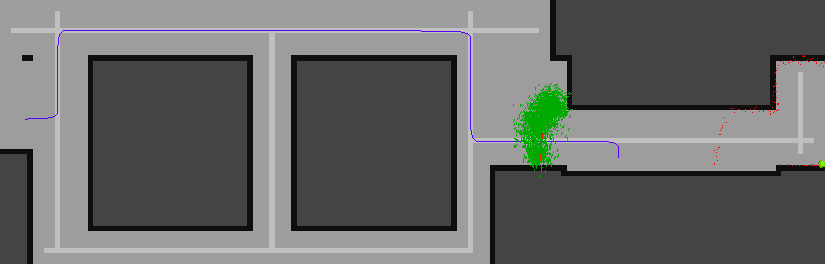
\includegraphics[scale=0.45]{images/pf_test_robot_stuck}
\caption{Particle Filter Test - Robot getting stuck}
\label{fig:pf_test_robot_stuck}
\end{figure}

The tests are carried out by running multiple simulations on the same map, and the success of a run is defined as a particle cluster formed around the robot with a variance among the particles below a certain threshold which triggers the path planning, and the robot planning a path to some location and successfully reaching this location, as shown in \autoref{fig:pf_test_success_a} and \ref{fig:pf_test_success_b}, respectively. If a particle cluster is formed at a wrong location and a path is planned from this location as in \autoref{fig:pf_test_not_found_following_path} and \autoref{fig:pf_test_robot_stuck}, this run is considered a failure.\\

\begin{figure}[H]
\centering

\begin{subfigure}{0.87\textwidth}
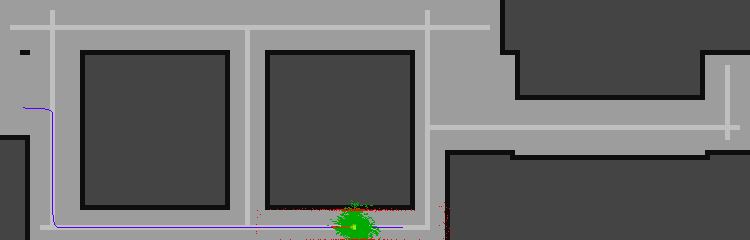
\includegraphics[width=\linewidth]{images/pf_test_following_path}
\caption{Robot following path}
\label{fig:pf_test_success_a}
\end{subfigure}

\hspace{\fill}

\begin{subfigure}{0.87\textwidth}
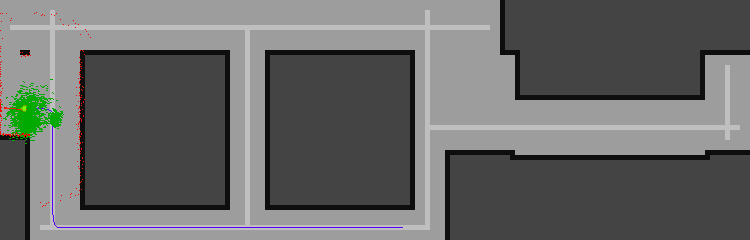
\includegraphics[width=\linewidth]{images/pf_test_reached_goal}
\caption{Robot reached goal}
\label{fig:pf_test_success_b}
\end{subfigure}

\caption{Particle Filter Test - Robot successfully located}
\label{fig:pf_test_success}
\end{figure}

Ten simulations have been conducted with the robot starting at the same location in each run and with the same goal for the path planning. Of these ten runs, six simulations resulted in robot successfully locating itself and reaching the goal. This of course works out to a success rate of 60\% which is not an impressive result. Whether this is acceptable or not depends on the application, but in most cases this probably won't be acceptable.

% section test (end)